\subsection{Neural Network Design and Training}
\label{subsec:nntraining}

%\begin{wrapfigure}{r}{0.5\textwidth}
%	\centering
%    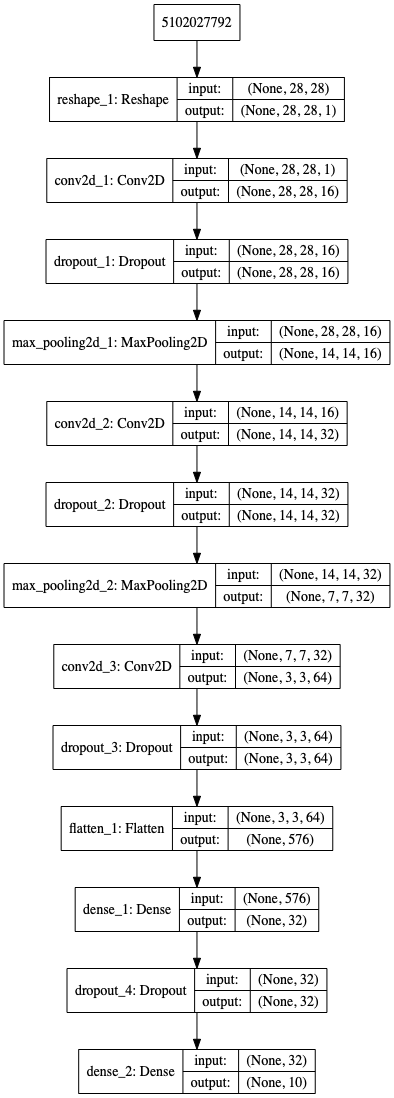
\includegraphics[width=0.35\textwidth]{img/nnlayout}
%	\caption{Network Layers}
%	\label{fig:network-layers}
%\end{wrapfigure}

The network was implemented in PyTorch \cite{Paszke:2019aa} as well as Tensorflow \cite{MartinAbadi:2015aa}. The backend was later exclusively switched to PyTorch (which is also the most common deep learning framework in Science) due to its better support of qunatization. The layers of the network can be seen in Figure~\ref{fig:network-layers}. 
For training of the network the \emph{ADAM} optimization algorithm \cite{Kingma:2014aa} was used to minimize the cross-entropy-loss function which is defined as
\begin{equation}
    J = - y  \log(h) + (1-y)  \log(1-h)
\end{equation}
For controlling the ADAM algorithm the recommended values, listed in Table~\ref{tab:train-params}, by \cite{Kingma:2014aa} was used.
\begin{table}[ht]
	\centering
    \caption{Network Training Parameters}
    \begin{tabular}{cc}
        \toprule
            Parameter & Value \\
        \midrule
            $\alpha$   & $0.001$ \\
            $\beta_1$  & $0.9$   \\
            $\beta_2$  & $0.999$  \\          
        \bottomrule
    \end{tabular}
    \label{tab:train-params}
\end{table}


A useful guide for implementing convolutions can be found in \cite{dumoulin2016guide}. The training 
of the network yielded very high accuracy rates - which is typical for the MNIST dataset, which is for
Machine Learning an easy challenge. Even though the network performance could be improved, e.g. by 
hyperparameter tuning the results were acceptable for our case. The progress of the training in terms
of accuracy and loss can be seen in Figure~\ref{fig:network-train-acc} respectively in Figure~\ref{fig:network-train-loss}.
The final output of the network over the training is evaluated in Figure~\ref{fig:network-test-cm} for real
values and in Figure~\ref{fig:network-test-qcm} for fake quantized values.

\begin{figure}[htbp]
	\centering
	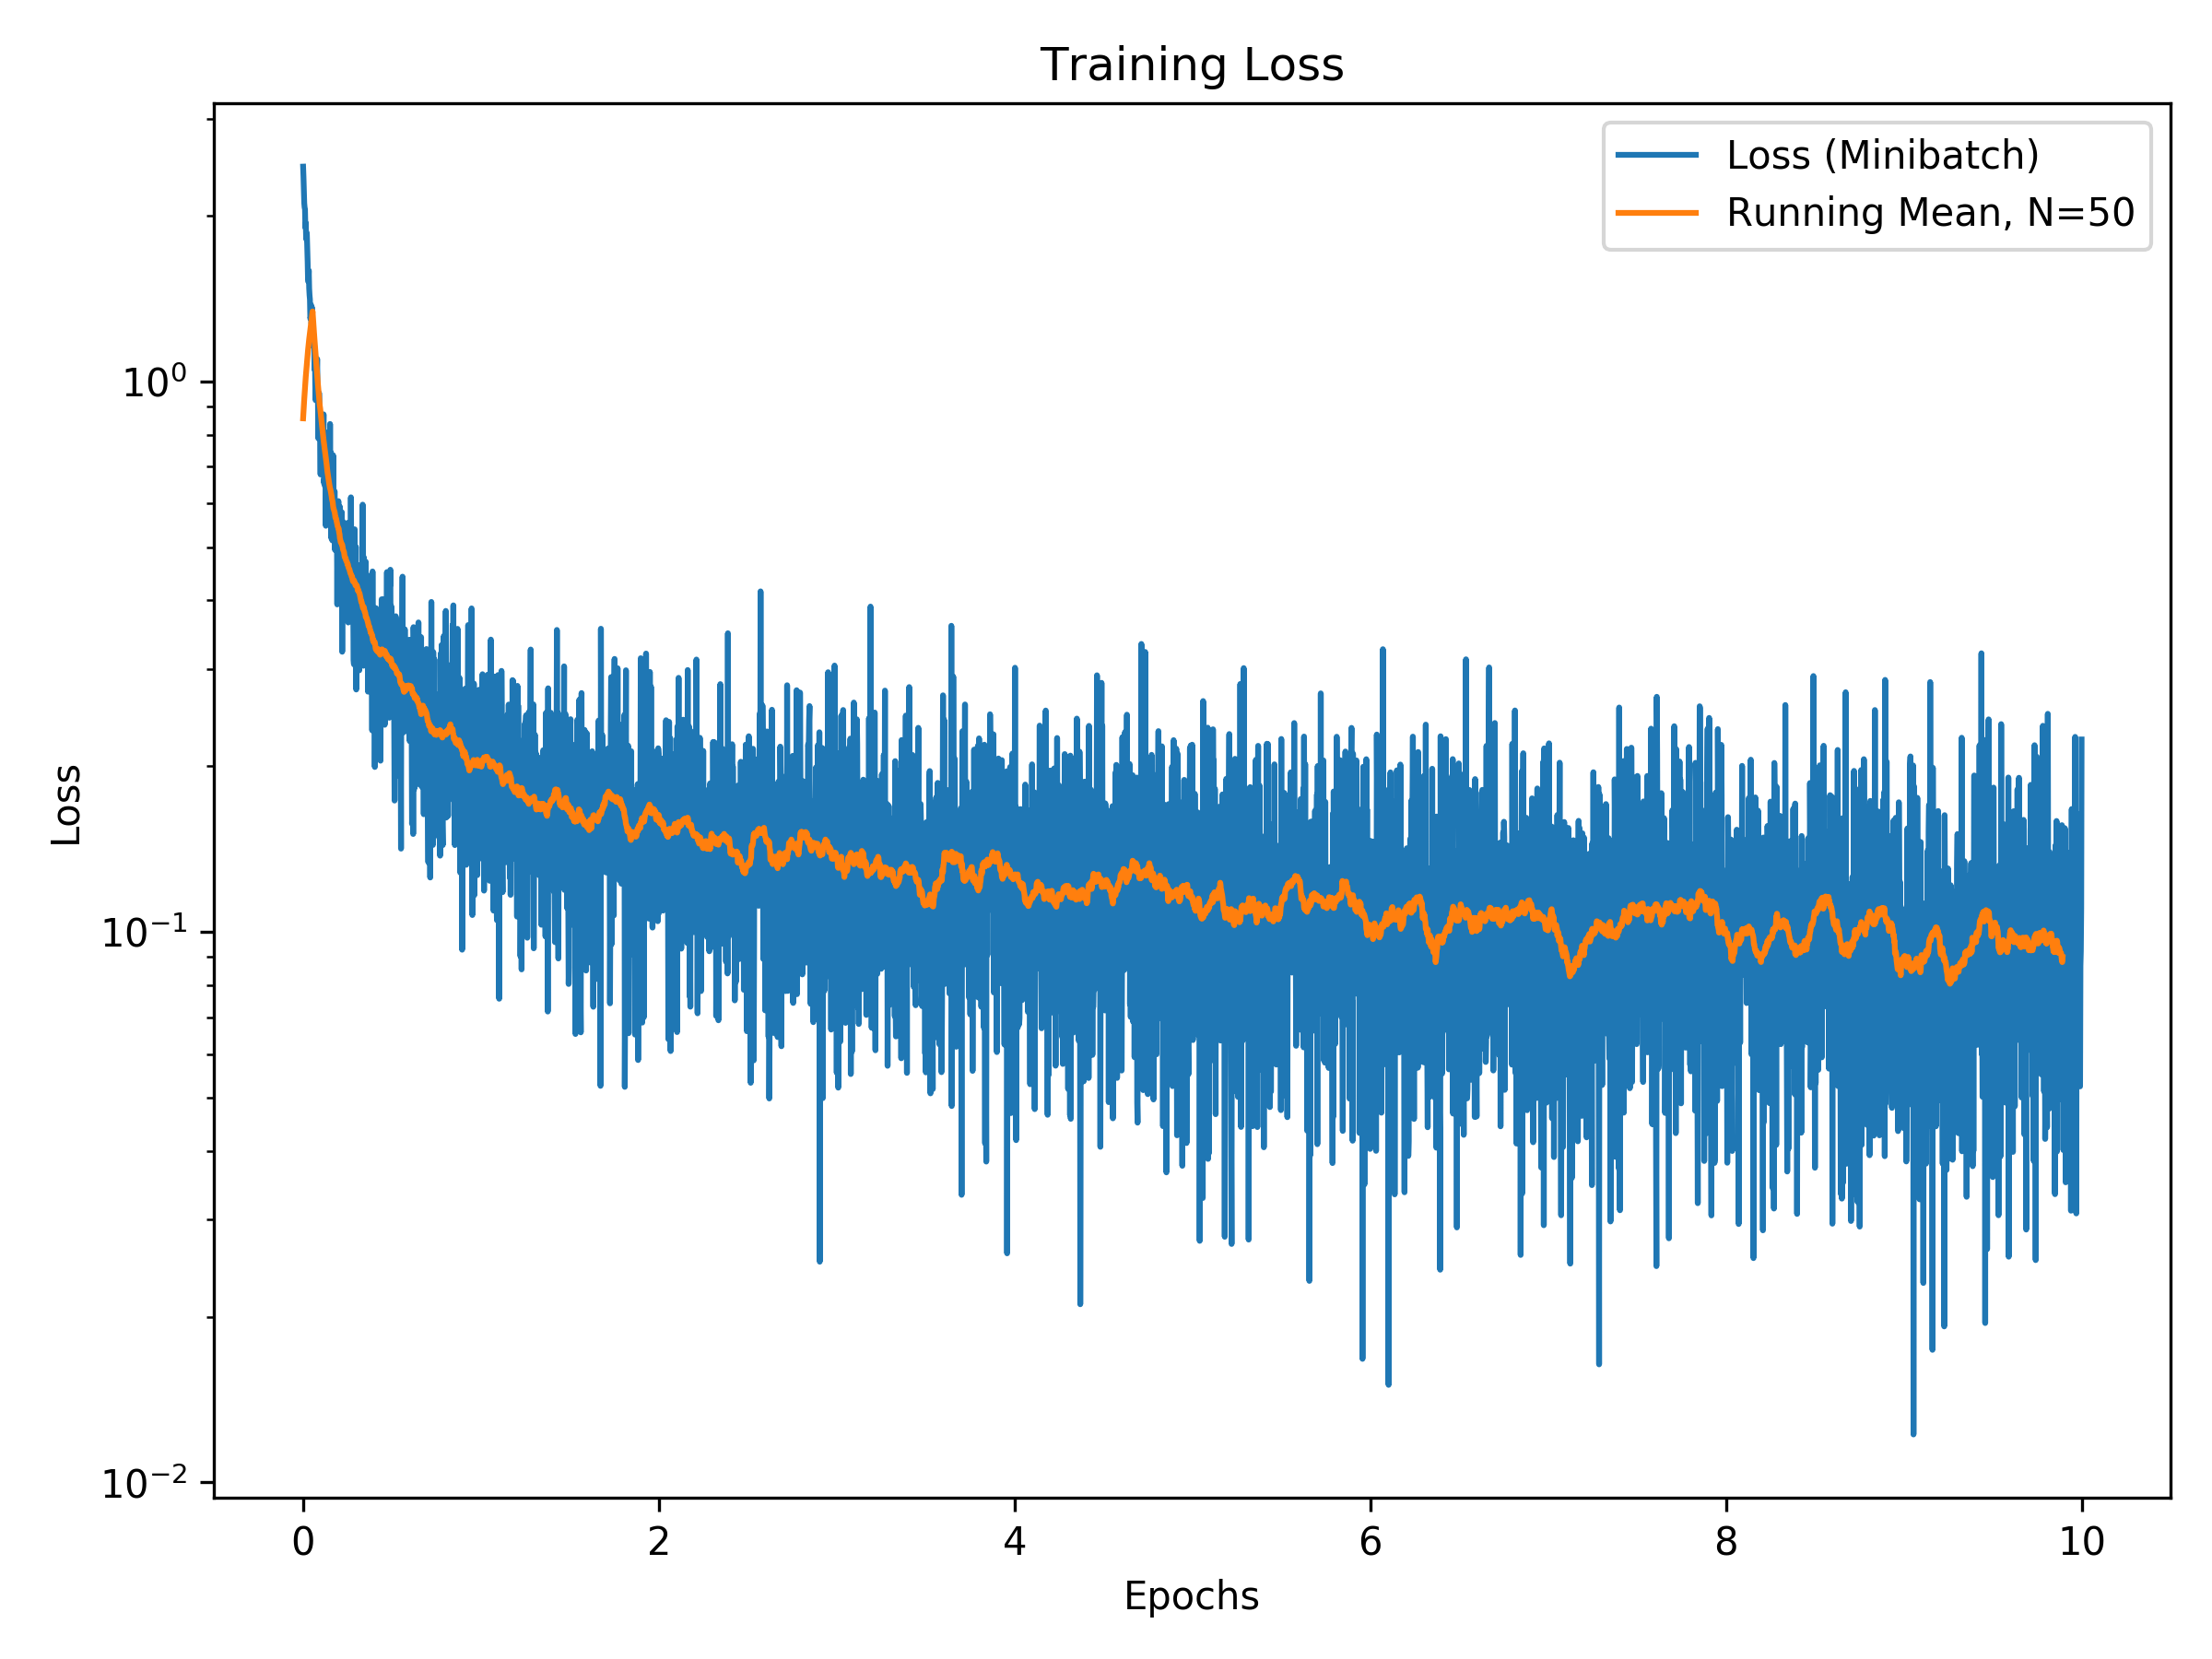
\includegraphics[width=0.8\textwidth]{../../net/images/training_loss}
	\caption{Training Loss}
	\label{fig:network-train-loss}
\end{figure}

\begin{figure}[htbp]
	\centering
	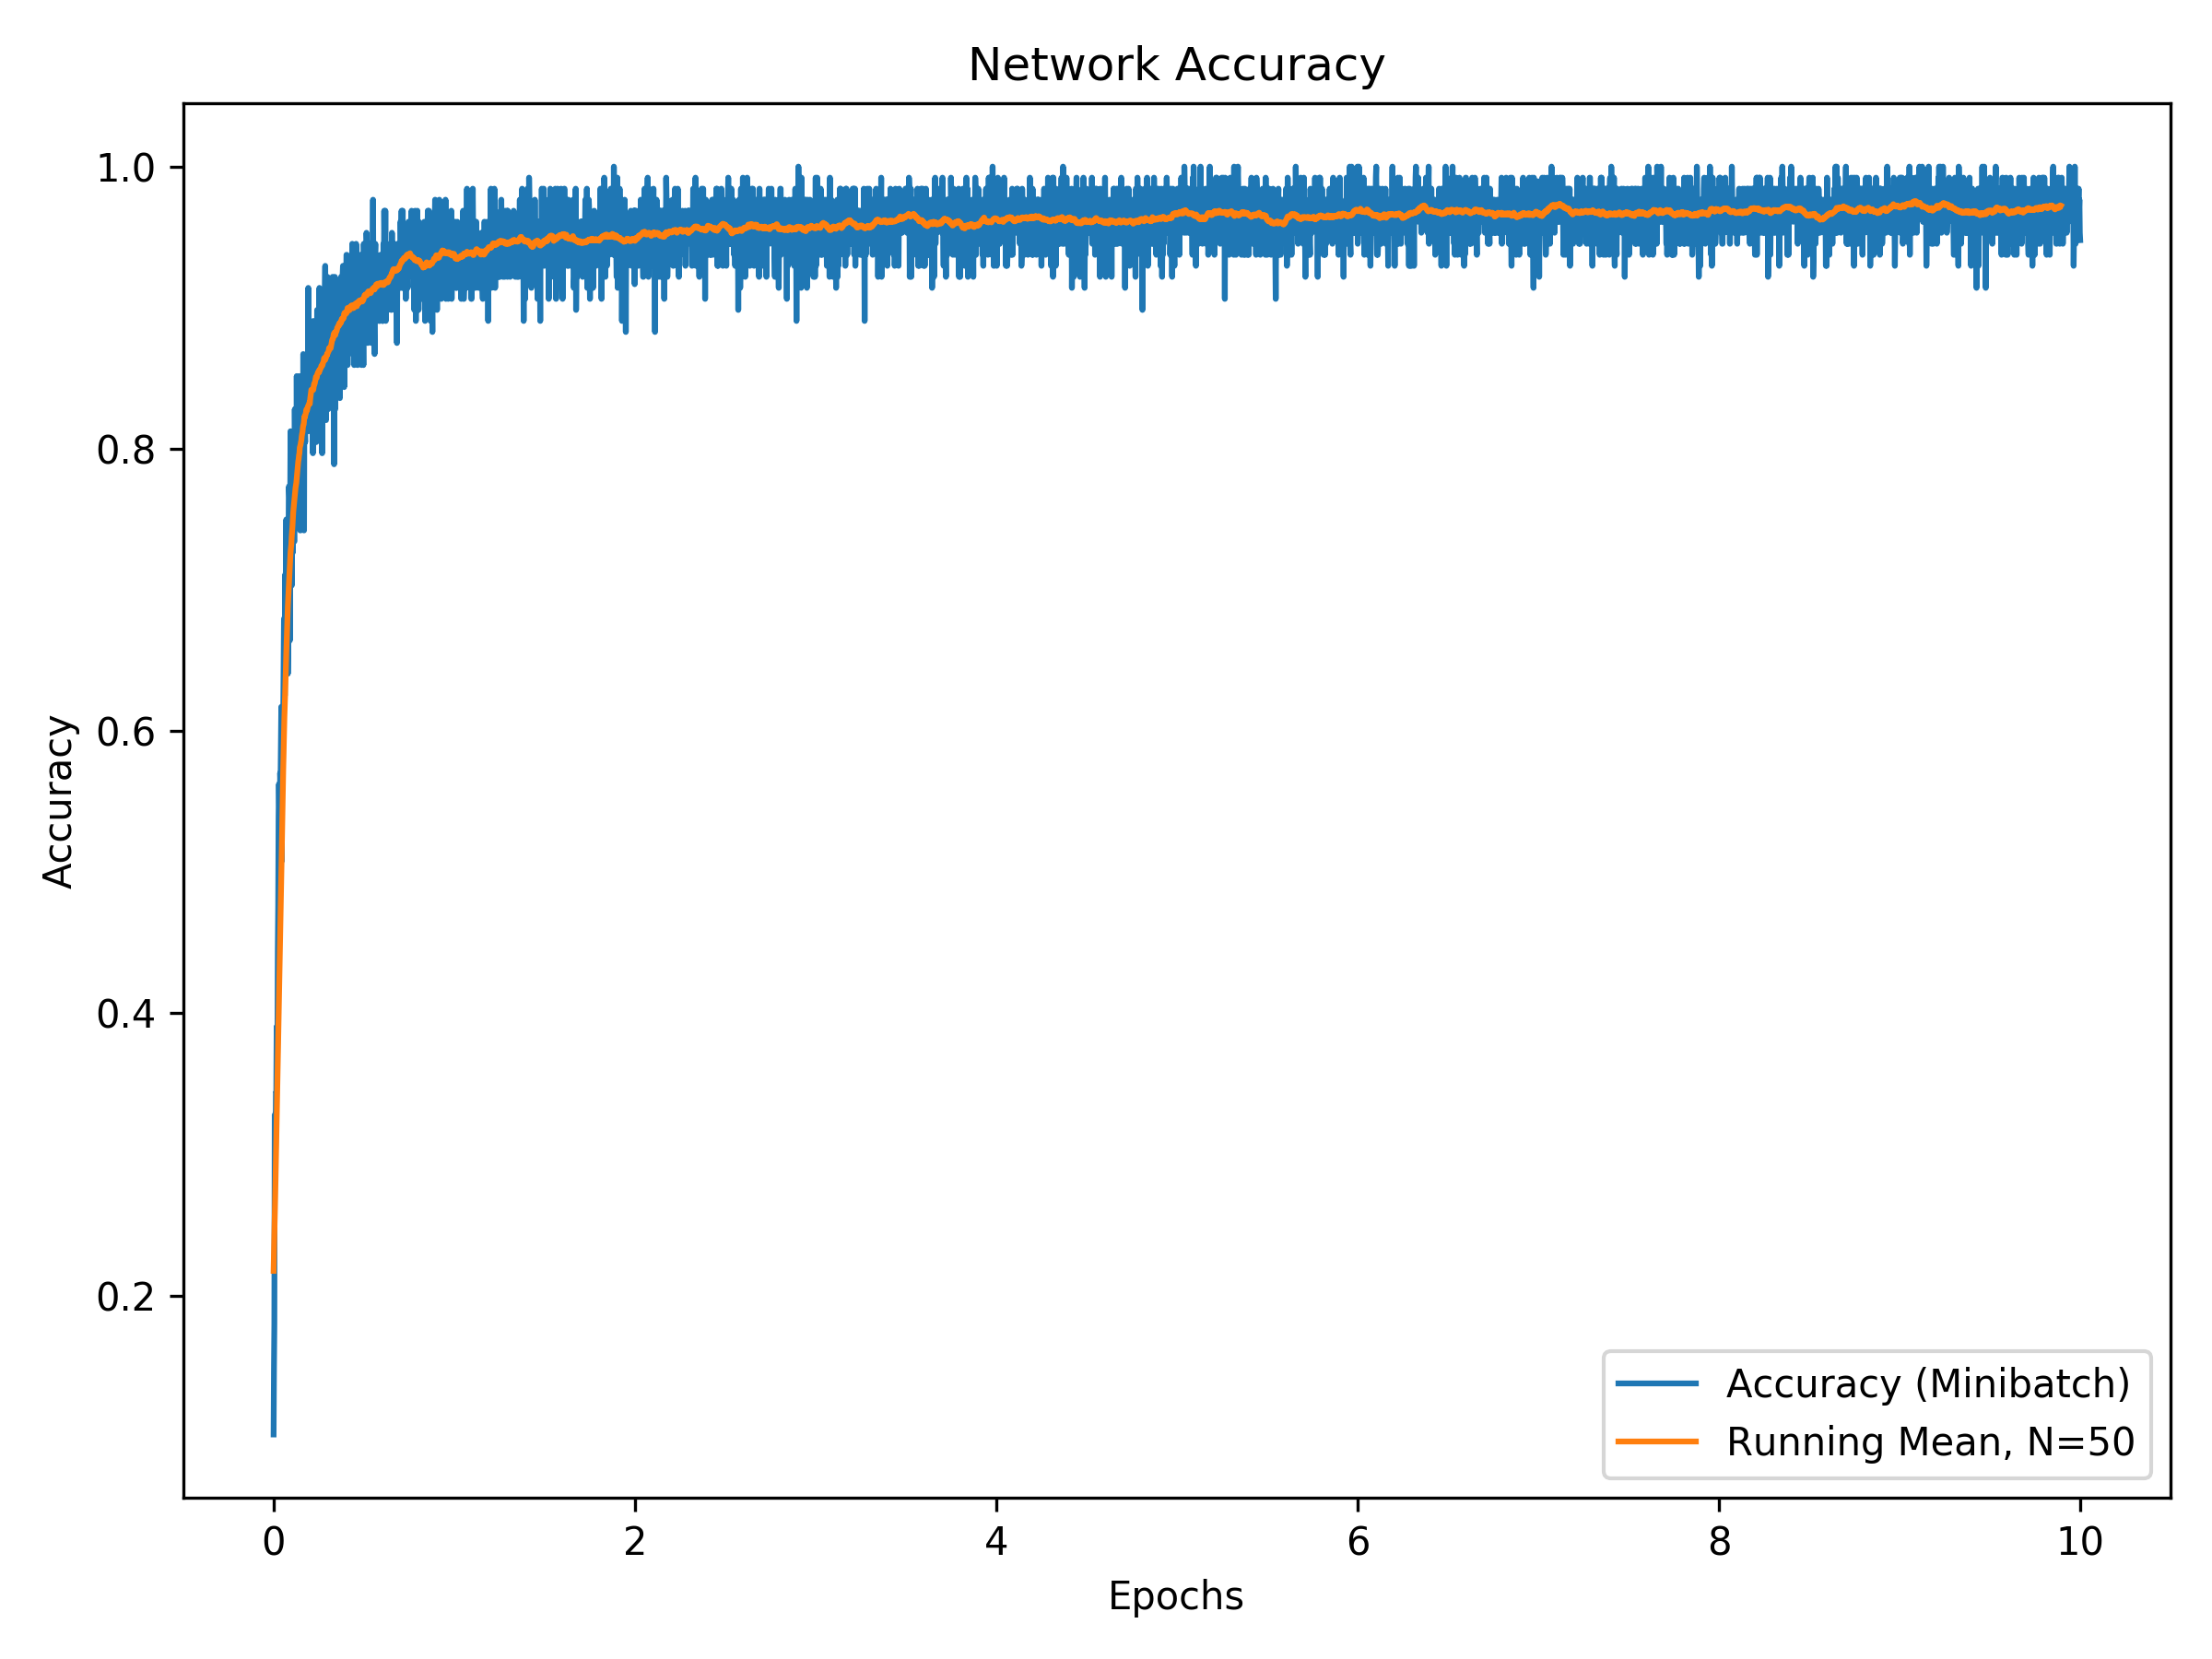
\includegraphics[width=0.8\textwidth]{../../net/images/training_accuracy}
	\caption{Training Accuracy}
	\label{fig:network-train-acc}
\end{figure}

\begin{figure}[htbp]
	\centering
	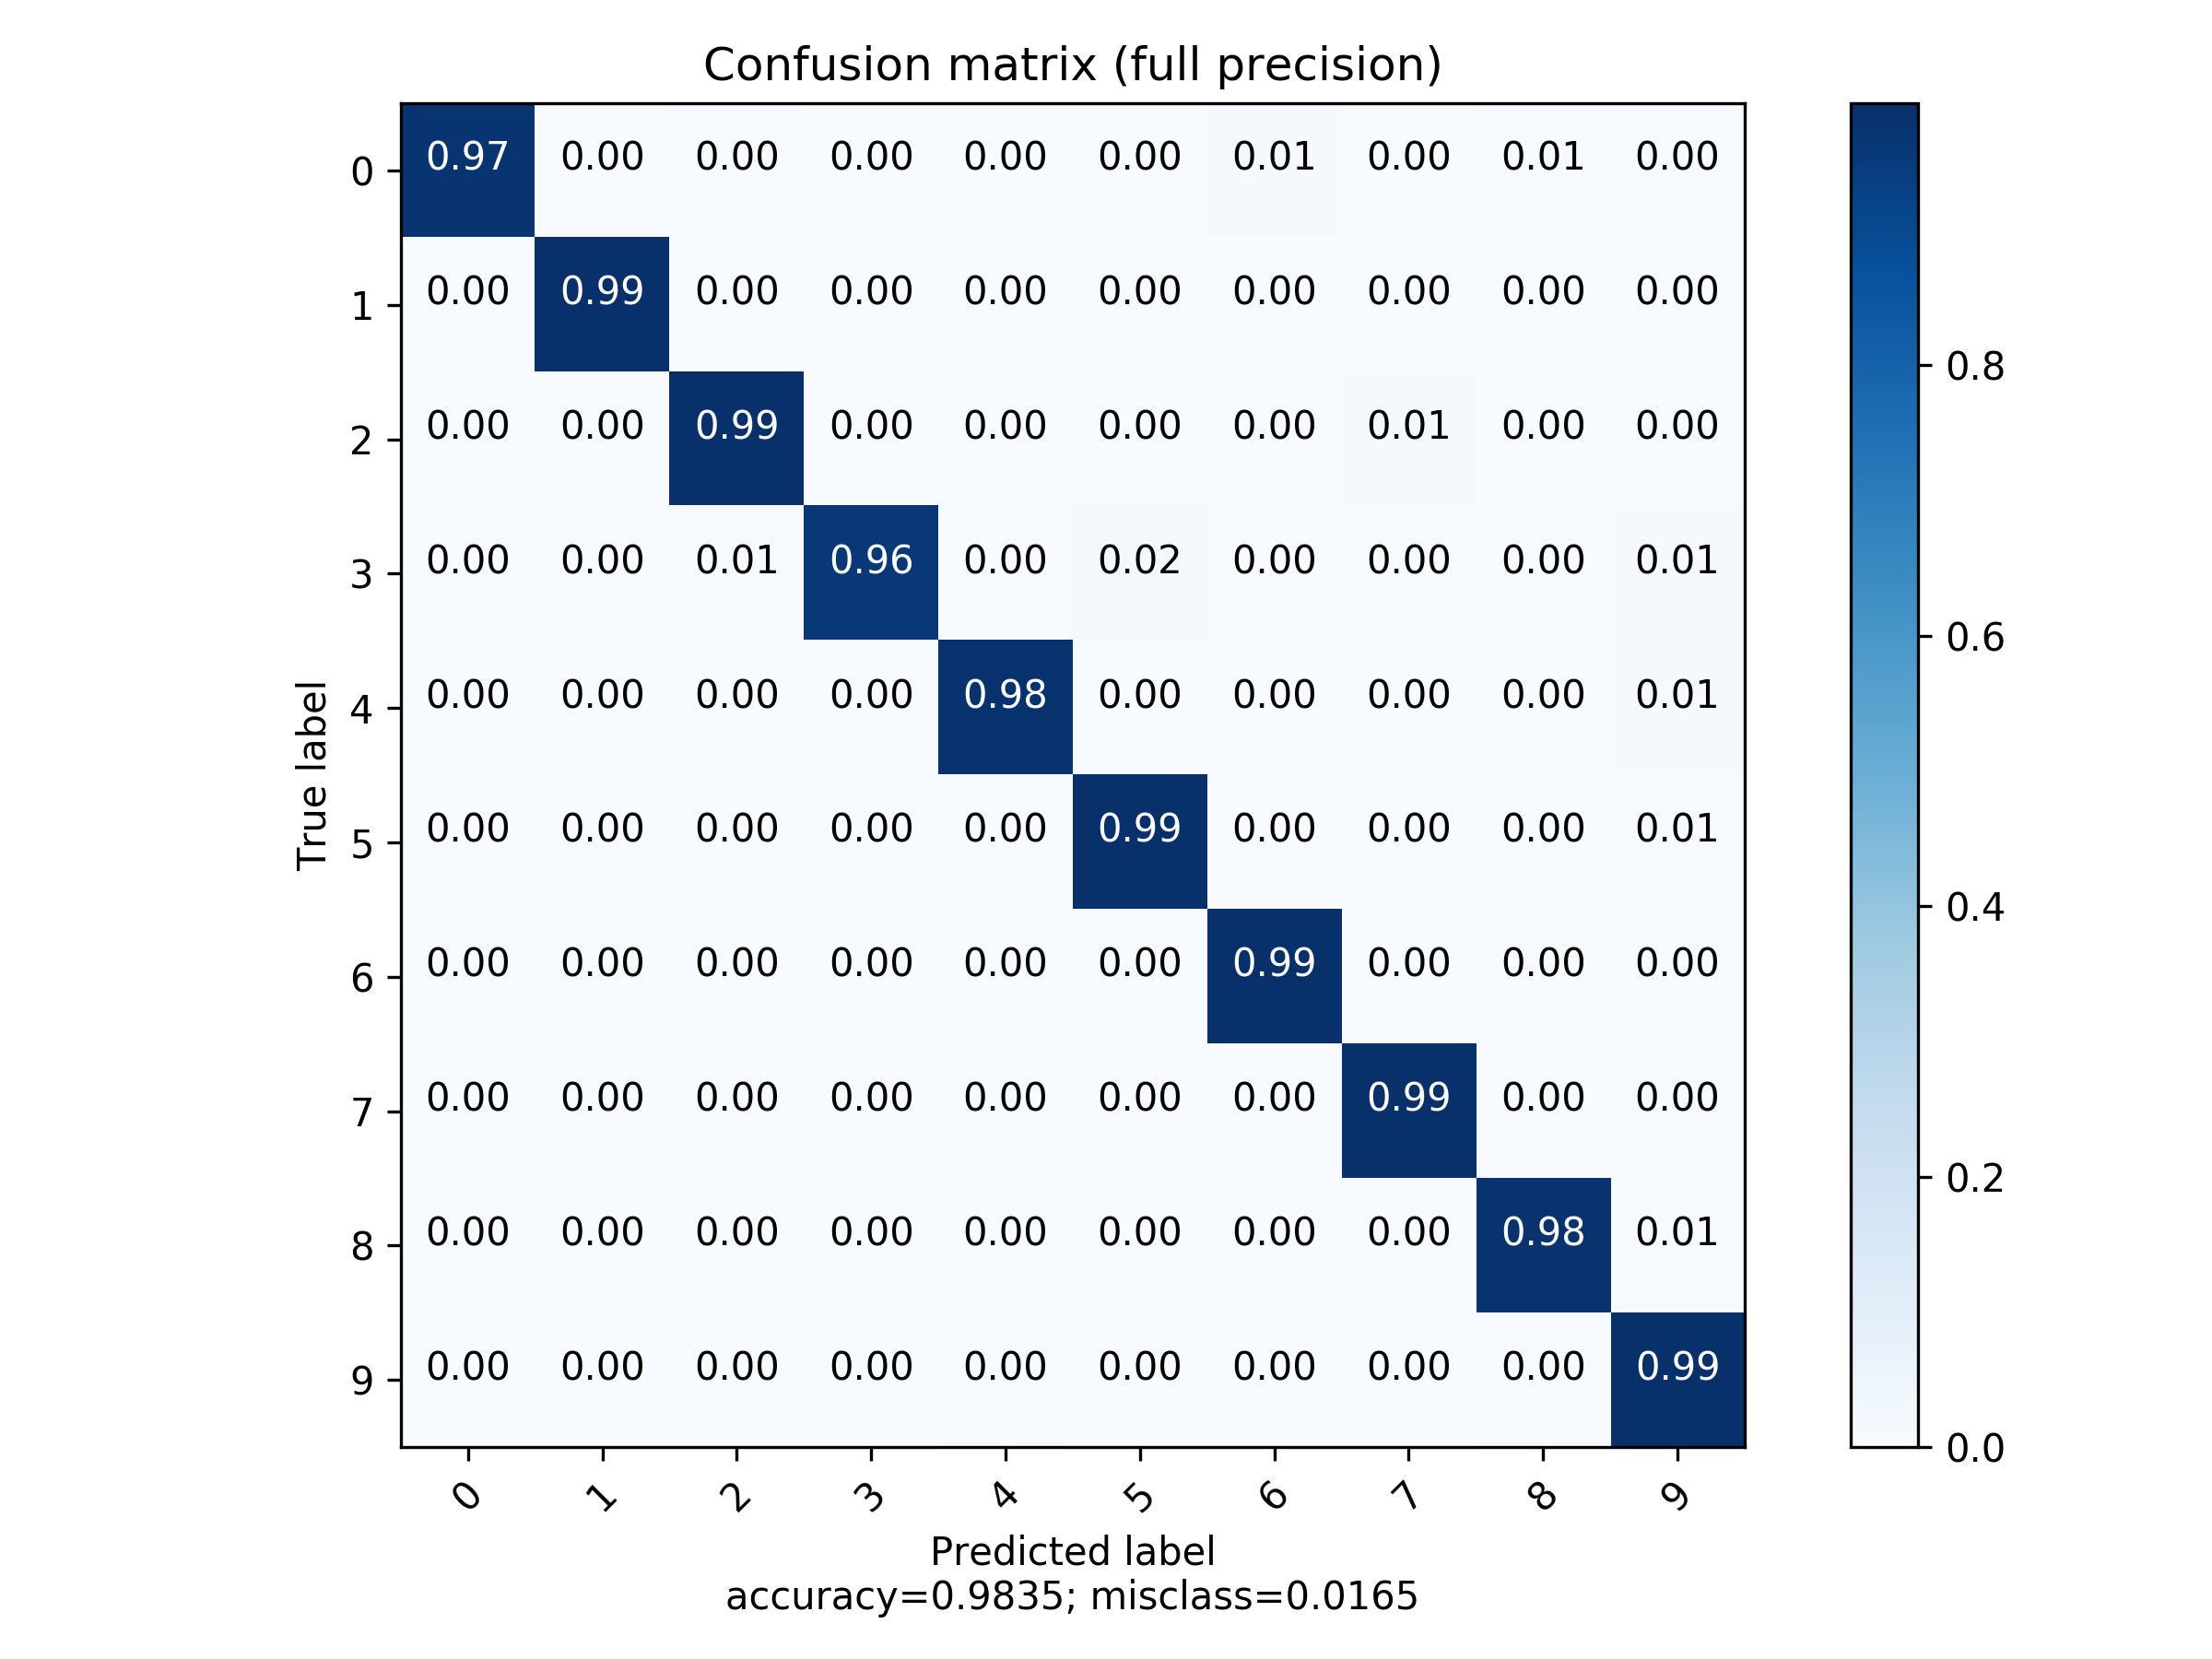
\includegraphics[width=0.8\textwidth]{../../net/images/cm}
	\caption{Confusion Matrix (real)}
	\label{fig:network-test-cm}
\end{figure}

\begin{figure}[htbp]
	\centering
	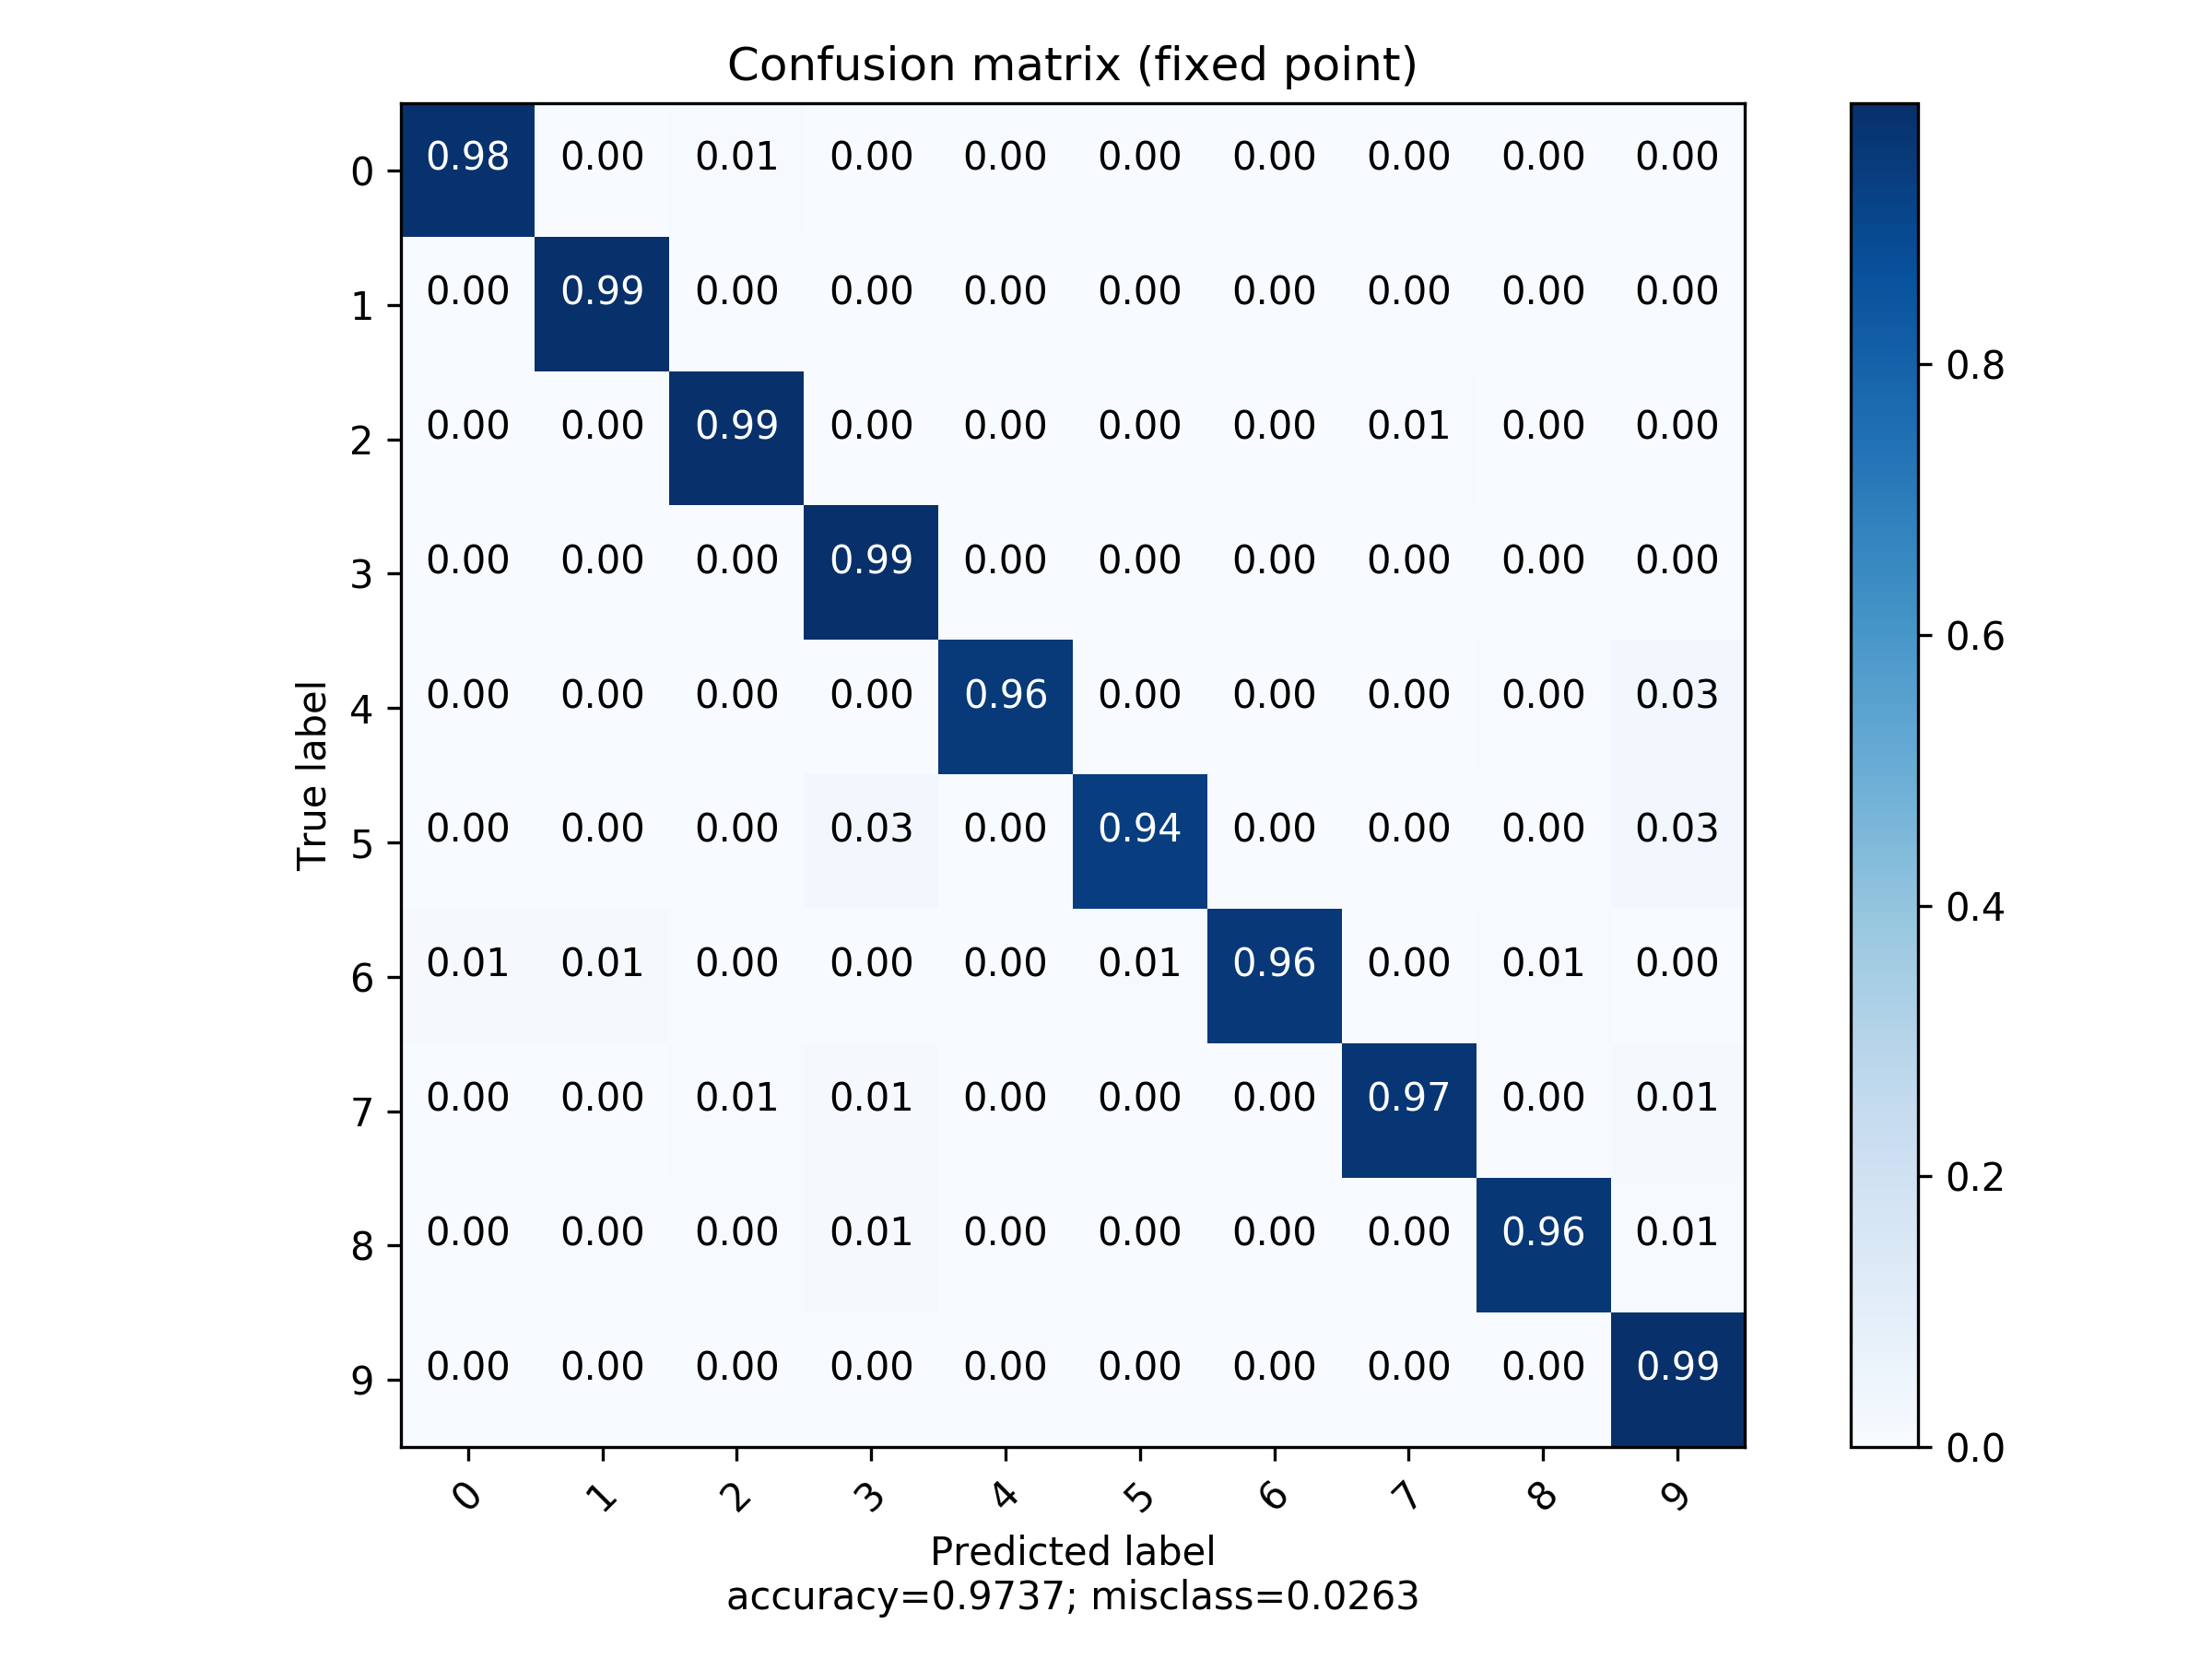
\includegraphics[width=0.8\textwidth]{../../net/images/qcm}
	\caption{Confusion Matrix with quantized values}
	\label{fig:network-test-qcm}
\end{figure}

\subsection{Quantization}

The network was reduced to fixed point integers defined by the equation
\begin{equation}
	v = Q \cdot 2 ^{-m}
\end{equation}
where both $Q$ and $m$ are integers and $v$ is the real value representation of the fixed point number. 
For our network implementation we chose a vairable fraction length for each layer and a total bitlength for $Q$ of $8$. 
This quantization can further be adjusted for each convolutional channel separately but optimization in this way were beyond the scope of this project.
The multiplication of two fixed point integers is trivial, because the product for two real values $v_1$ and $v_2$ is 
\begin{equation}
	v_1 v_2 = \text{right-shift}\left( Q_1 Q_2 \cdot 2^{-(m+m)} ; m\right)
\end{equation}
In our tests a quantization with $8$ bit fixedpoint integers and even $4$ bit integers showed only a small drop in accuracy of around $1 \%$.
\todo{Add Histogram}


